

\section{CV-VTON+} \label{section:cpvton+}

\subsection{Overview} 

Fig. 4 illustrates the new pipeline emphasizing the modifications from CP-VTON, which tackles all 4 issues above mentioned except extreme 3D pose of target human.

\begin{itemize}

\item Correction on the cloth agnostic representation   


\begin{itemize}

\item Modification 1: We added a new label ‘Skin’ to the human parsing data to represent the human body shape more accurately (Fig. 2. (a) right).

\item Modification 2: We removed the hair label from the Reserved Regions of GMM’s Person Representation input, i.e. only face remains.  

\end{itemize}


\item Un-changed human area inclusion  

\begin{itemize}
\item Modification 3: We added extra human components except the target cloth area, e.g. bottom clothes and legs in the Reserved Regions of Person Representation to TOM, along with face and hair (Fig. 2. (b) right).

\end{itemize}

\item Improving Composition alpha-map 


\begin{itemize}

\item Modification 4: In the mask loss term in TOM loss function, we replaced the Composition Mask with supervised ground truth mask for a strong alpha mask.

\begin{equation}
L=c_1 |I_0-I_{GT} |+  c_2 L_{VGG}+c_1 |M_{GT}-M_0 |       
\end{equation}

\item Modification 5: Lastly, we added the binary mask of warped cloth to TOM network input so that TOM can clearly differentiate the target cloth area regardless of cloth color.  

\end{itemize}

\item GMM improvement Will be here: GIC loss and Mask ETC


The previous image based VTON algorithms use geometric matching and transform model  of Roccos et al. \cite{rocco2017convolutional}, which again uses the spatial transform networks by Zimmerman et al.'s \cite{jaderberg2015spatial}. Although warping network can work in both instance-level and category-level, our experiments  reveals the warped cloth often distorted severely. We try to understand the original of the misbehaivors, but failed to do. Our finding is that the warping network try to matches cloth images with human representation of silhouette and joint heatmap. The latter does not have no texture features but the shape information. From the failure case examinations, we found that the warping in the failure case is often too extreme, so that we try to restrict the warping parameters. Instead of single step TPS warping, we designed 2 stage warping network, in the first stage it warped roughly with Affine transform, and in the second stage it warped delicately with TPS transform. Not to have un-realistic warping, we added warping regularization loss. In the second stage, the sizes of cloth and target area in the human representation are in the same scale, so that the matching network can find the matching better. 

\begin{equation}
 L_{gridreg} (G_x, G_y) = sum_x sum_y | G_x(x+1, y) - G_x(x, y) | + | G_x(x, y) - G_x(x-1, y) | + | G_x(x, y+1) - G_x(x, y) | + | G_x(x, y) - G_x(x, y-1) |
\end{equation}


In the experiment section, we will describe the effects of 2 stage method and regularization method.
 
   
Thai Write here the details for design and figure.


Thai Write the experimental results in the next section

\end{itemize}


\begin{figure}
\centering
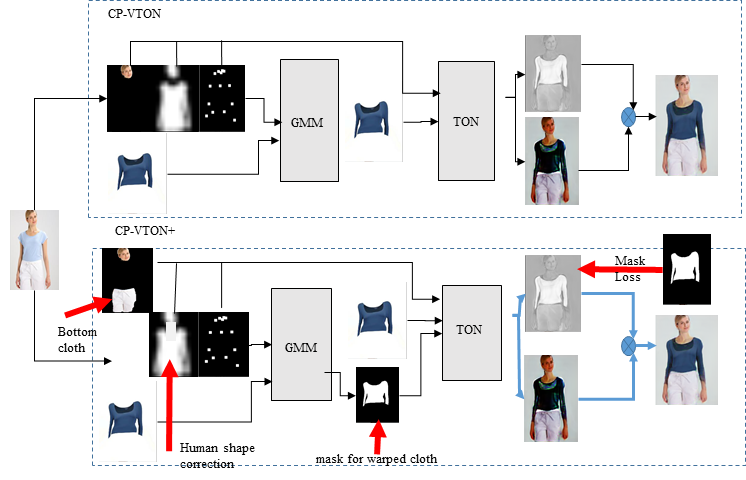
\includegraphics[height=6.5cm, scale=1]{figures/cpvton+pipeline.png}   
\caption{Full pipeline Comparison: CP-VTON and CP-VTON+}
\label{fig:piepline}
\end{figure}

\begin{figure}
\centering
%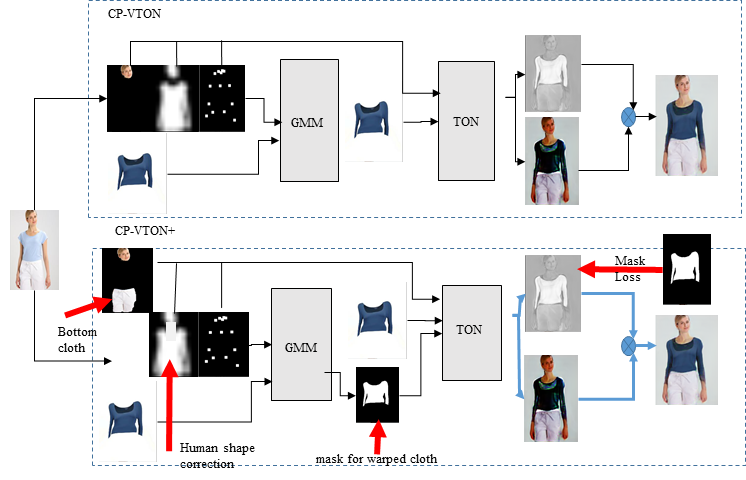
\includegraphics[height=6.5cm, scale=1]{figures/cpvton+pipeline.png}   
\caption{2 stage GMM design with regularization loss}
\label{fig:piepline}
\end{figure}

